\subsection{Apposition Surface Plugin}

An apposition surface is the planar surface that best fit the structure of a
segmentation.\\

Apposition Surface Plugin provides three-dimensional representation of
segmentation's apposition surface. Therefore, the following button is available
in three-dimensional views.\\

\vspace{0.3cm}

\desc{Show Apposition Surface}{../../frontend/rsc/appPlane}
{Display segmentation's apposition surface}

\begin{figure}[H]
  \label{Fig:color_tracking}
  \subfigure[Original Segmentation]{
     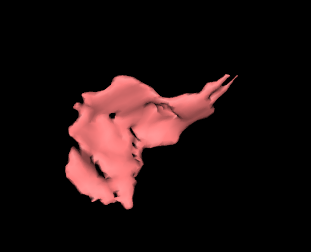
\includegraphics[width=0.3\linewidth]{fig/AppSurface-seg}
  }
  \hfill
  \subfigure[Apposition Surface]{
    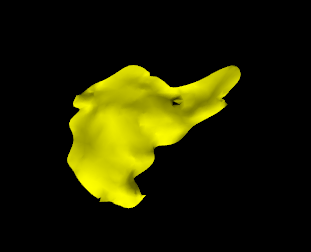
\includegraphics[width=0.3\linewidth]{fig/AppSurface-surface}
    }
  \hfill
  \subfigure[Superimposed representations]{
    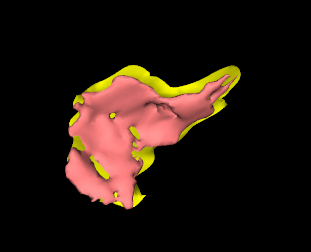
\includegraphics[width=0.3\linewidth]{fig/AppSurface-surface-seg}
  }
\caption{Segmentatio and Apposition Surface 3D meshes.}
\end{figure}

In addition, it provides the apposition surface area and perimeter information
to segmentations.\\

\begin{figure}[H]
\centering
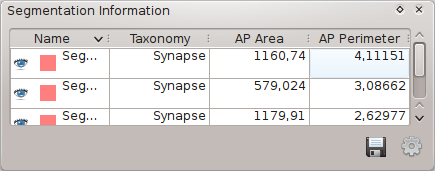
\includegraphics{fig/AppSurface-info}
\caption{Information provided by Appsition Surface Plugin.}
\end{figure}
